%%%%%%%%%%%%%%%%%%%%%%%%%%%%%%%%%%%%%%%%%%%%%%%%%%%%%%%%%%%%%%%%%%%%%%%%%%%%%%%%
% Medium Length Graduate Curriculum Vitae
% LaTeX Template
% Version 1.2 (3/28/15)
%
% This template has been downloaded from:
% http://www.LaTeXTemplates.com
%
% Original author:
% Rensselaer Polytechnic Institute 
% (http://www.rpi.edu/dept/arc/training/latex/resumes/)
%
% Modified by:
% Daniel L Marks <xleafr@gmail.com> 3/28/2015
%
% Important note:
% This template requires the res.cls file to be in the same directory as the
% .tex file. The res.cls file provides the resume style used for structuring the
% document.
%
%%%%%%%%%%%%%%%%%%%%%%%%%%%%%%%%%%%%%%%%%%%%%%%%%%%%%%%%%%%%%%%%%%%%%%%%%%%%%%%%

%-------------------------------------------------------------------------------
%	PACKAGES AND OTHER DOCUMENT CONFIGURATIONS
%-------------------------------------------------------------------------------

%%%%%%%%%%%%%%%%%%%%%%%%%%%%%%%%%%%%%%%%%%%%%%%%%%%%%%%%%%%%%%%%%%%%%%%%%%%%%%%%
% You can have multiple style options the legal options ones are:
%
%   centered:	the name and address are centered at the top of the page 
%				(default)
%
%   line:		the name is the left with a horizontal line then the address to
%				the right
%
%   overlapped:	the section titles overlap the body text (default)
%
%   margin:		the section titles are to the left of the body text
%		
%   11pt:		use 11 point fonts instead of 10 point fonts
%
%   12pt:		use 12 point fonts instead of 10 point fonts
%
%%%%%%%%%%%%%%%%%%%%%%%%%%%%%%%%%%%%%%%%%%%%%%%%%%%%%%%%%%%%%%%%%%%%%%%%%%%%%%%%

\documentclass[margin]{res}  
\usepackage[spanish]{babel}
\selectlanguage{spanish}
\usepackage[utf8]{inputenc}

% Default font is the helvetica postscript font
\usepackage{helvet}

% Increase text height
\textheight=700pt

\usepackage{graphicx}
\usepackage{multirow}

\begin{document}

%-------------------------------------------------------------------------------
%	NAME AND ADDRESS SECTION
%-------------------------------------------------------------------------------
\name{Ivan Dario Echeverry Mancera} 
\address{\multirow{0}{*}{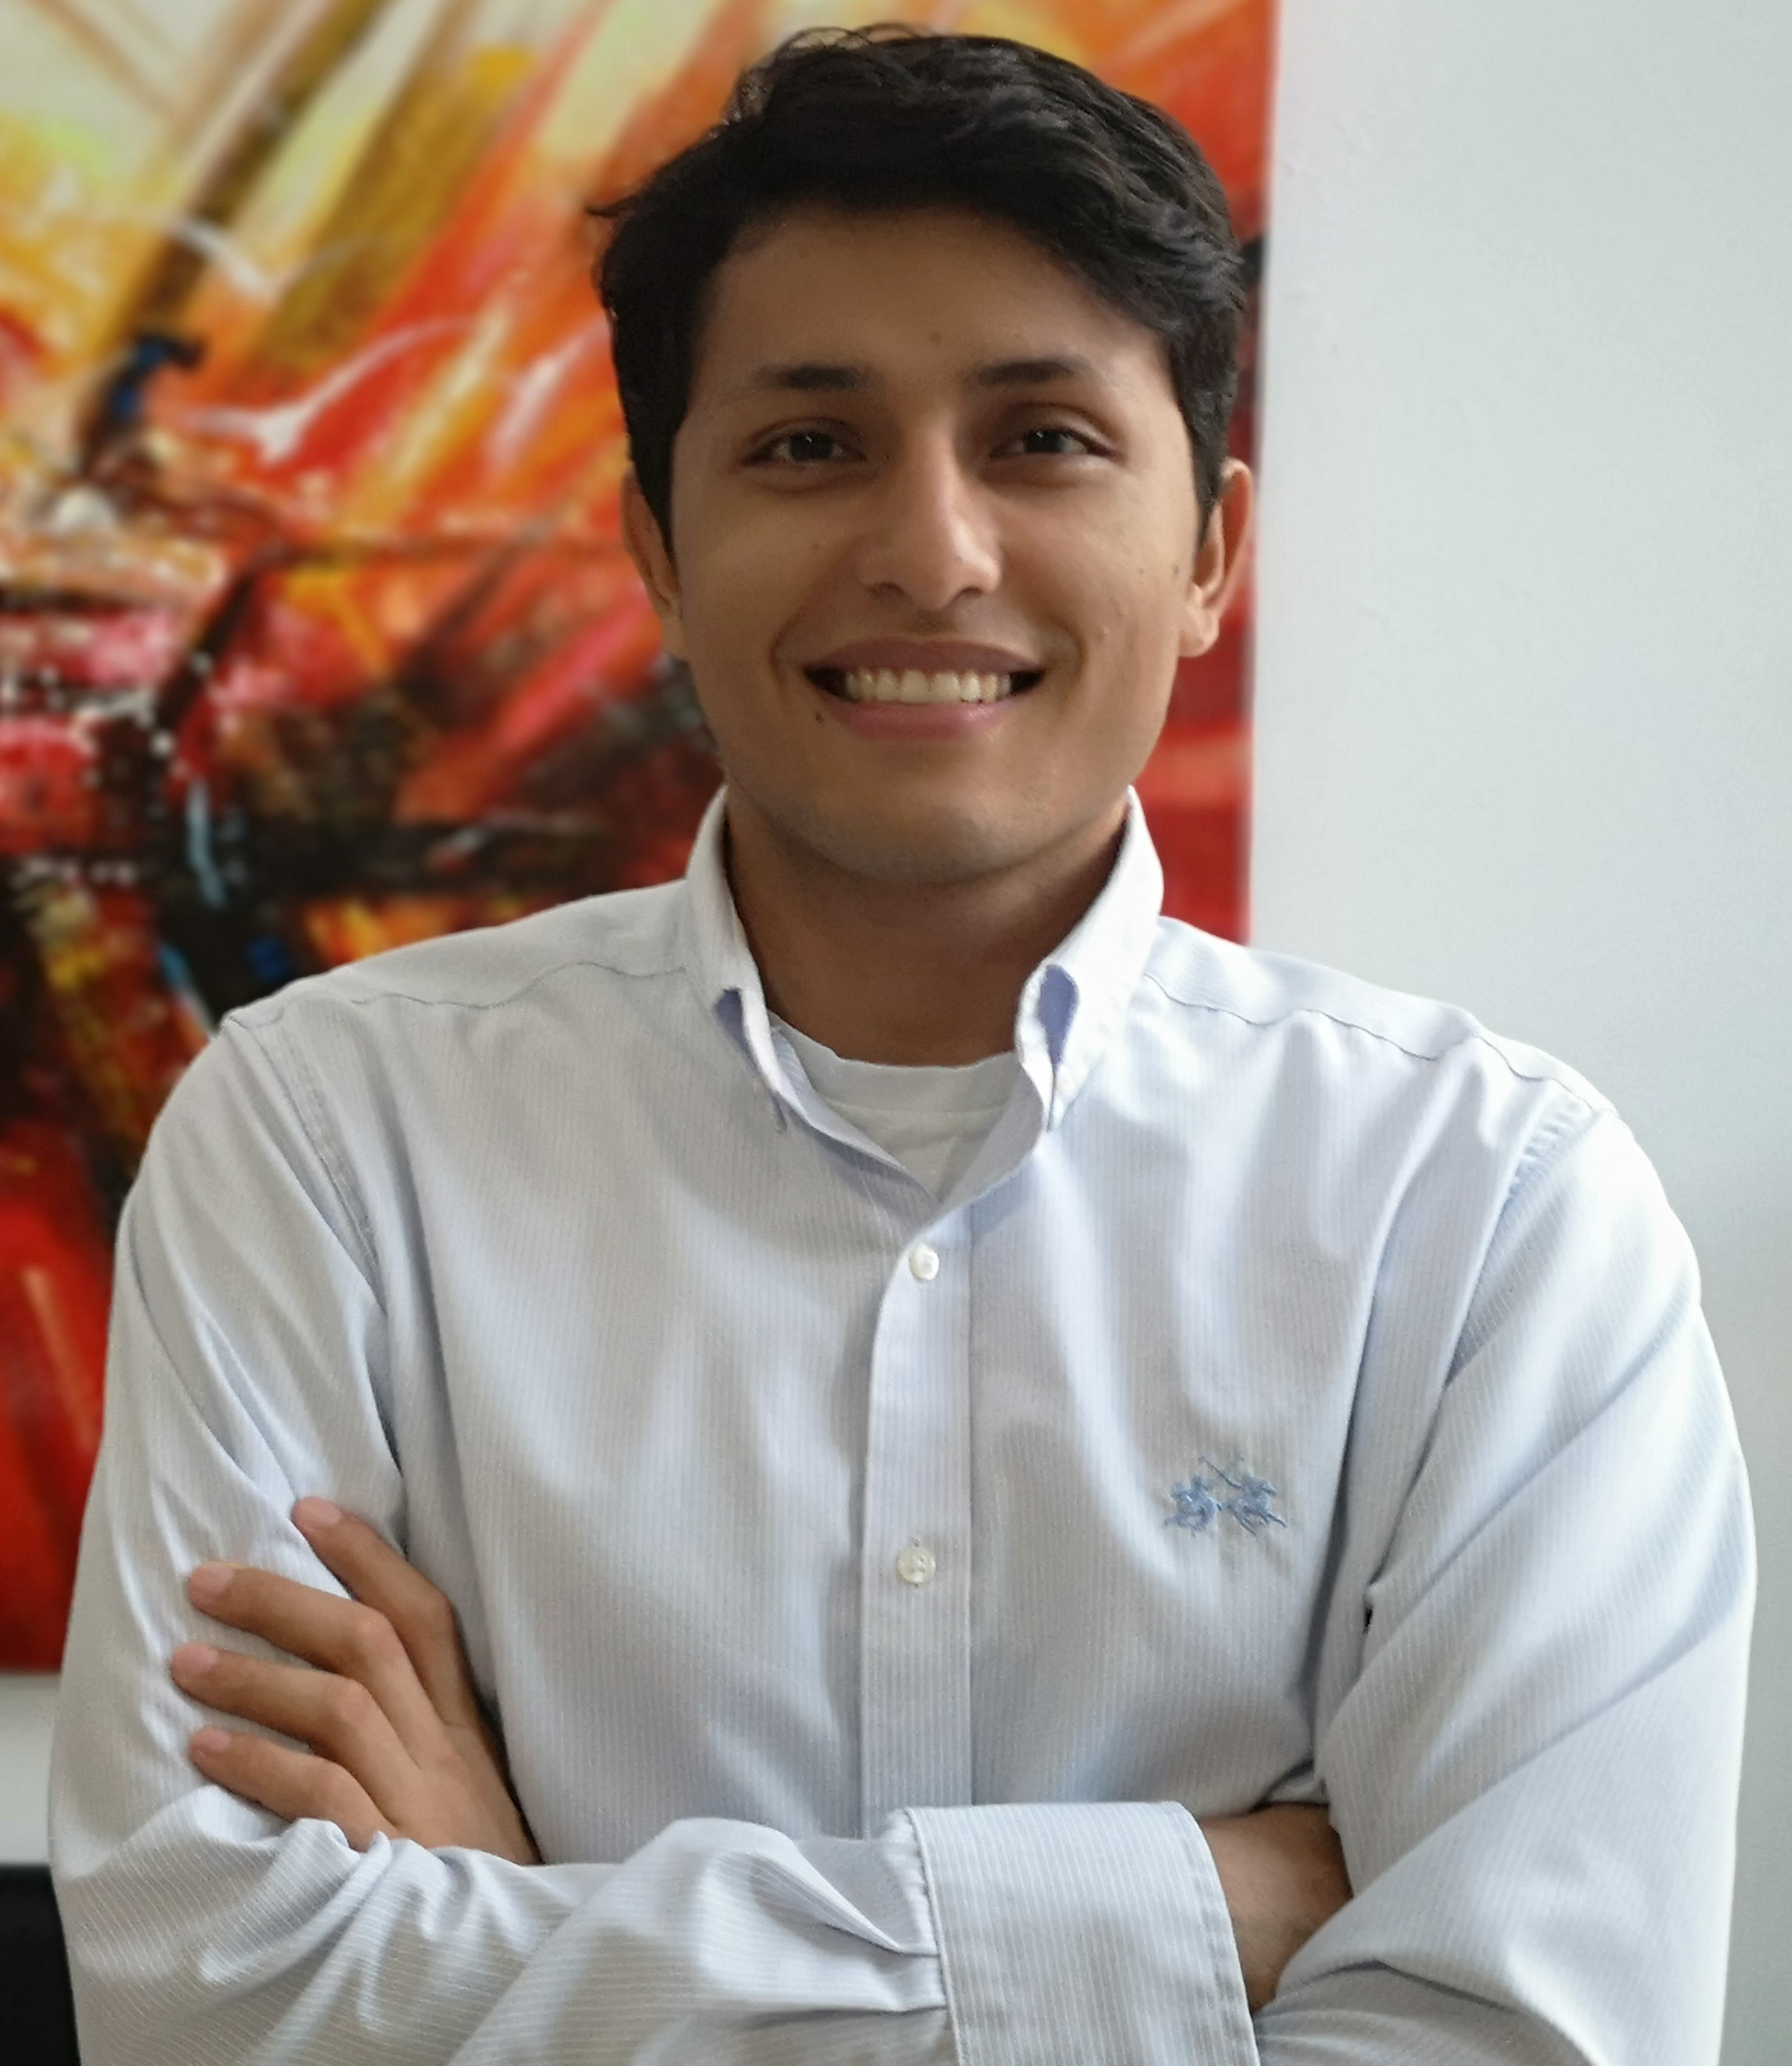
\includegraphics[width=3.4cm]{FOTO}}}
% * <mrigou@itba.edu.ar> 2015-12-23T16:08:16.140Z:
%
% ^.

% Note that addresses can be used for other contact information:
% -phone numbers
% -email addresses
% -linked-in profile

% Simulate as if there are 7 lines of address
\address{\\\\\\\\29 - Marzo - 1992\\ Ingeniero Electrónico y Electricista\\C.C.: 1.096.219.233
\\Lugar de Expedición: Barrancabermeja\\Cel: +57-3005762828
\\Correo: echeverry9203@gmail.com\\Cartagena, Bolívar}
% Hence the photo would take 7 lines/rows
%\address{\multirow{4}{*}{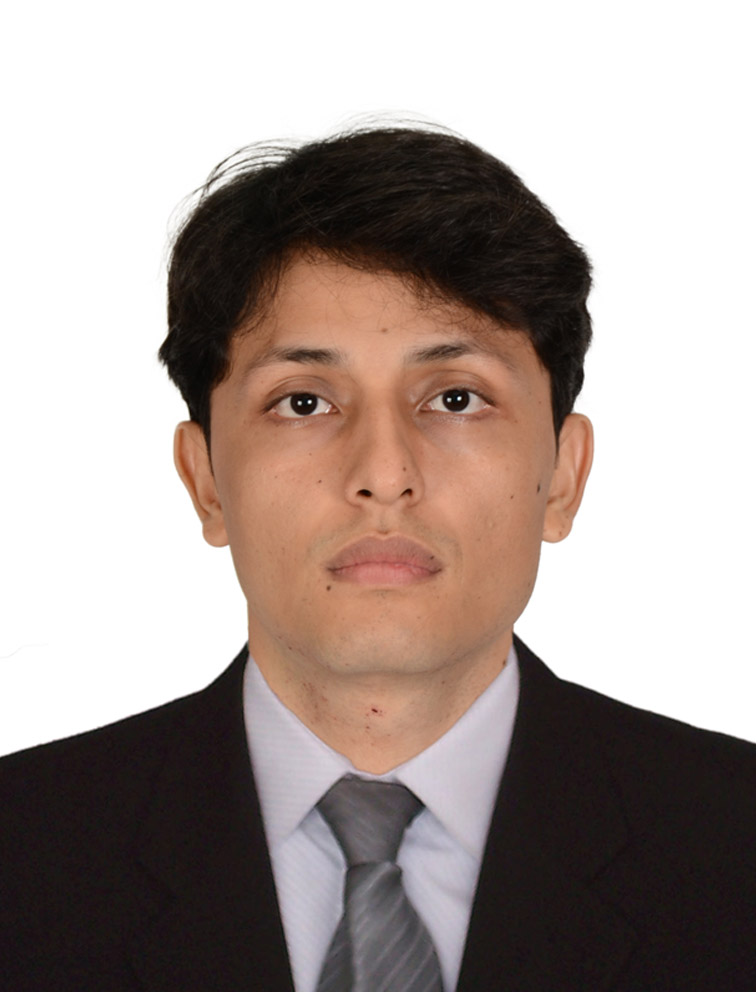
\includegraphics[width=2.5cm]{CVFOTO}}}

% Uncomment to add a third address
%\address{Address 3 line 1\\Address 3 line 2\\Address 3 line 3}
%-------------------------------------------------------------------------------

\begin{resume}

%-------------------------------------------------------------------------------
%	EDUCATION SECTION
%-------------------------------------------------------------------------------
\section{RESUMEN}
Ingeniero Electrónico y Electricista de la Universidad Tecnológica de Bolívar con dos años de experiencia laboral en Ingeniería. Gran capacidad de comunicación y de resolución de problemas.

\section{EDUCACIÓN}
\textbf{UTB}, Universidad Tecnológica de Bolívar\\
{\sl \textbf{Ingeniería Eléctrica}} \hfill Junio 2017 - Octubre 2020
\\
{\sl Proyecto de grado: Caso de estudio Descargas Parciales, Industria cementera.}
\\\\
\textbf{UTB}, Universidad Tecnológica de Bolívar\\
{\sl \textbf{Ingeniería Electrónica}} \hfill Enero 2011 - Julio 2017
\\
{\sl Proyecto de grado: Diseño electrónico para una plantilla que mide los niveles de presión en distintos puntos de la zona plantar.}
\\\\
\textbf{Secundaria}, Colegio Militar Almirante Colon \hfill Graduación: Dic-2010
\\
\textbf{Técnicos}, Colegio Militar Almirante Colon\\
{\sl Técnico en Administración y Comercio} \hfill Graduación: Dic-2010

%-------------------------------------------------------------------------------

%-------------------------------------------------------------------------------
%	PROJECTS SECTION
%-------------------------------------------------------------------------------
\section{EXPERIENCIA}

\section{\multirow{0}{*}{
\includegraphics[width=2.3cm]{logoHELIOS}}\centering}
\hfill \break
\textbf{Helios Consulting S.A.S.}: \hfill Agosto 2020 - Actualidad
\\Ingeniería Eléctrica y Electrónica.
\\Medidas de aislamiento en cables de media tensión XLPE con tensiones nominales de 13.8kV - Medidas de sistemas de puesta a tierra – Medidas descargas parciales en celdas de media tensión, análisis y elaboración de reportes técnicos – Monitoreo y análisis de Calidad de energía en motores, celdas de transformadores y tableros de baja tensión - Manejo de bases de datos.

\section{\multirow{0}{*}{
\includegraphics[width=1.8cm]{Proctek_logo.png}}\centering}
\hfill \break
\textbf{Proctek Process Control Technologies}: \hfill Julio 2020
\\ Ingeniero Electrónico.
\\Visitas técnicas para el levantamiento de base instalada Rockwell Automation.

\section{\multirow{0}{*}{
\includegraphics[width=1.3cm]{logoKWH}}\centering}
\hfill \break
\textbf{KWH Ingeniería S.A.S.}: \hfill Febrero 2020 - Julio 2020
\\Ingeniería Eléctrica y Electrónica.
\\Planeacion de instalación para un interruptor de 115kV en MS Project - Diseño de instalaciones eléctricas en media tensión - Estudio y curvas para Coordinación de protecciones - Estudio de Arco eléctrico. 

\newpage

\section{\multirow{0}{*}{
\includegraphics[width=2.3cm]{logoHELIOS}}\centering}
\hfill \break
\textbf{Helios Consulting S.A.S.}: \hfill Noviembre 2018 - Enero 2020
\\Ingeniería Eléctrica y Electrónica.
\\Medidas de sistemas de puesta a tierra – Medida de resistividad del terreno – Medidas descargas parciales en celdas de media tensión, análisis y elaboración de reportes técnicos - Medición de Campos electromagnéticos – Monitoreo y análisis de Calidad de energía en motores, celdas de transformadores y tableros de baja tensión - Manejo de bases de datos - Balances de Materia y Energía 

\section{\multirow{0}{*}{
\includegraphics[width=1.8cm]{logoGEISCOL}}\centering}
\hfill \break
\textbf{Global Energy Innovations Solutions Colombia S.A.S.}: \hfill Mayo 2019 - Julio 2019
\\ Ingeniero Electricista.
\\Diseño eléctrico del escenario deportivo Estadio de Béisbol 11 de noviembre Cartagena - Seguimiento de proyecto - Levantamiento del sistema eléctrico para el diseño - Elaboración y presentación de reportes a contratistas - Elaboración de presupuestos en obra eléctrica.

\section{\multirow{0}{*}{
\includegraphics[width=1.3cm]{logoKWH}}\centering}
\hfill \break
\textbf{KWH Ingeniería S.A.S.}: \hfill Enero 2019 - Junio 2019
\\Pasantía – Ingeniería Eléctrica.
\\Elaboración de presupuestos para obras eléctricas - Levantamiento de instrumentación electrónica - Estudio para Coordinación de protecciones - Estudio de Arco eléctrico - Diseño eléctrico para bodegas. 

\section{\multirow{0}{*}{
\includegraphics[width=1.3cm]{unnamed.jpg}}\centering}
\hfill \break
\textbf{Hotel Caribe}: \hfill Agosto 2017 - Febrero 2018
\\Pasantía – Ingeniería Electrónica.
\\Programacion de rutinas de mantenimiento de equipos - Documentación de consumos de servicios públicos - Apoyo gestión de oficina, activos de almacén - Supervisión y ejecución de trabajos con personal técnico - Apoyo distribución de labores de trabajo al personal de turno - Entrega de reportes técnicos al personal encargado para su diligenciamiento e ingreso a su respectiva hoja de vida - elaboración de procedimientos de actividades o manejo de equipos donde se requiera. 

%\par
%\textbf{Profesora Particular}: \hfill 2007 - 2014 
%\\
%Matemáticas, Física y Química para estudiantes de secundaria y primer año de universidad.

%-------------------------------------------------------------------------------
%-------------------------------------------------------------------------------
%	Interests
%-------------------------------------------------------------------------------
%\newpage
\section{CURSOS}

\section{\multirow{0}{*}{
\includegraphics[width=2.7cm]{RA_Logo.jpg}}\centering}
\hfill
\\\textbf{CCP143 Studio 5000 Logix Designer Level 3:} \hfill Junio 24 del 2020
\\Project Development.
\\ 9 horas. Rockwell Automation.

%\section{\multirow{0}{*}{
\includegraphics[width=2.7cm]{RA_Logo.jpg}}\centering}
%\hfill
\\\textbf{CCCL21 Studio 5000 Logix Designer Level 3:} \hfill Junio 22 del 2020
\\Basic Ladder Logic Interpretation.
\\ 4 horas. Rockwell Automation.

%\section{\multirow{0}{*}{
\includegraphics[width=2.7cm]{RA_Logo.jpg}}\centering}
%\hfill
\\\textbf{CCP151 Studio 5000 Logix Designer Level 2:} \hfill Junio 21 del 2020
\\Basic Ladder Logic Programming.
\\ 4 horas. Rockwell Automation.

%\section{\multirow{0}{*}{
\includegraphics[width=2.7cm]{RA_Logo.jpg}}\centering}
%\hfill
\\\textbf{CCP146 Studio 5000 Logix Designer Level 1:} \hfill Junio 19 del 2020
\\ControlLogix Logix 5000 System Fundamentals.
\\ 7 horas. Rockwell Automation. 

\section{\multirow{0}{*}{
\includegraphics[width=2.6cm]{aciem-bolivar.png}}\centering}
\hfill
\\\textbf{Interventoria en Obras Eléctricas.} \hfill Julio 2019
\\ 16 horas. ACIEM Bolívar. 

\section{\multirow{0}{*}{
\includegraphics[width=2.5cm]{logo_megger.jpg}}\centering}
\hfill
\\\textbf{Conceptos y Experiencias en la Medición de Descargas Parciales en Redes Energizadas.} 
\\ Certificado de Asistencia. Webinar Megger. \hfill Junio 2019

\section{\multirow{0}{*}{
\includegraphics[width=2.6cm]{aciem-bolivar.png}}\centering}
\hfill
\\\textbf{Diseño Detallado de la A a la W.} \hfill Febrero 2019
\\16 horas. ACIEM Bolívar.

\section{\multirow{0}{*}{
\includegraphics[width=1.5cm]{Cisco_CCNA.png}}\centering}
\hfill
\\\textbf{CCNA Switching \& Routing: Conexión de redes.}\hfill Agosto - Octubre 2016
\\240 horas. Universidad del Norte. 

\\\textbf{CCNA Switching \& Routing: Escalamiento de redes.} \hfill Junio - Julio 2016
\\210 horas. Universidad del Norte. 

\\\textbf{CCNA Switching \& Routing: Principios básicos de routing y switching.}
\\240 horas. Universidad del Norte. \hfill Abril - Junio 2016

\\\textbf{CCNA Switching \& Routing: Introducción a redes.}\hfill Febrero - Abril 2016
\\216 horas. Universidad del Norte. 

\\\textbf{XII Encuentro Departamental de Semilleros de Investigación EDESI.}
\\Ponente, 16 horas. Universidad San Buenaventura. \hfill Febrero - Mayo 2015


\section{\multirow{0}{*}{
\includegraphics[width=1.3cm]{logo_sena.jpg}}\centering}
\hfill
\\\textbf{Controladores Lógicos Programables PLC I.}\hfill Febrero - Diciembre 2012
\\40 horas. SENA. 

%-------------------------------------------------------------------------------
%	COMPUTER SKILLS SECTION
%-------------------------------------------------------------------------------
\hfill
\section{IDIOMAS}

\begin{itemize}
  \item Inglés,  (Básico) \hfill Leer (X), Escribir (X), Hablar(-)

\end{itemize}

\section{SOFTWARE}
Microsoft Office, Avanzado. Incluye Access y MS Project.\\
Software de diseño: AUTOCAD 2D Avanzado, Solidworks 3D, Altium, MATLAB, Studio 5000 Logix Designer\\
Simuladores de Sistemas de Potencia: ETAP 16, DigSilent.\\
De Texto: \LaTeX básico.


%-------------------------------------------------------------------------------

%-------------------------------------------------------------------------------
%	EXPERIENCE SECTION
%-------------------------------------------------------------------------------
% Modify the format of each position
%\begin{format}
%\title{l}\employer{r}\\
%\dates{l}\location{r}\\
%\body\\
%\end{format}
%-------------------------------------------------------------------------------

%\section{EXPERIENCE}
%\employer{Department for the Regulation and Control of Magical Creatures}
%\location{Location One}
%\dates{Dates One}
%\title{\textbf{Junior Officer}}
%\begin{position}
%Vivamus ullamcorper a lacus non laoreet. Etiam ultricies in est quis finibus. 
%Curabitur posuere est quis felis sodales, vitae aliquam ex consequat. In non 
%magna felis.
%\end{position}

%\employer{Employer One}
%\location{Location One}
%\dates{Dates One}
%\title{\textbf{Title One}}
%\begin{position}
%Donec venenatis volutpat tortor, quis fringilla turpis ornare et. Curabitur 
%\end{position}

%-------------------------------------------------------------------------------
%	Interests
%-------------------------------------------------------------------------------
\section{HABILIDAD PROFESIONAL}
Diseño y Construcción de tarjetas electrónicas de control y potencia con entradas y salidas digitales, análogas y comunicación para ser programadas desde un PC, diseñadas de acuerdo a la necesidad de la aplicación para el control de variables de proceso como temperatura, presión, nivel, flujo, corriente; aplicado al control secuencial de bombas, control de nivel de tanques, controladores solares, sobretensión y baja tensión en baterías.
\\

%-------------------------------------------------------------------------------
\end{resume}

%\newpage
%\begin{figure*}
%\centering
%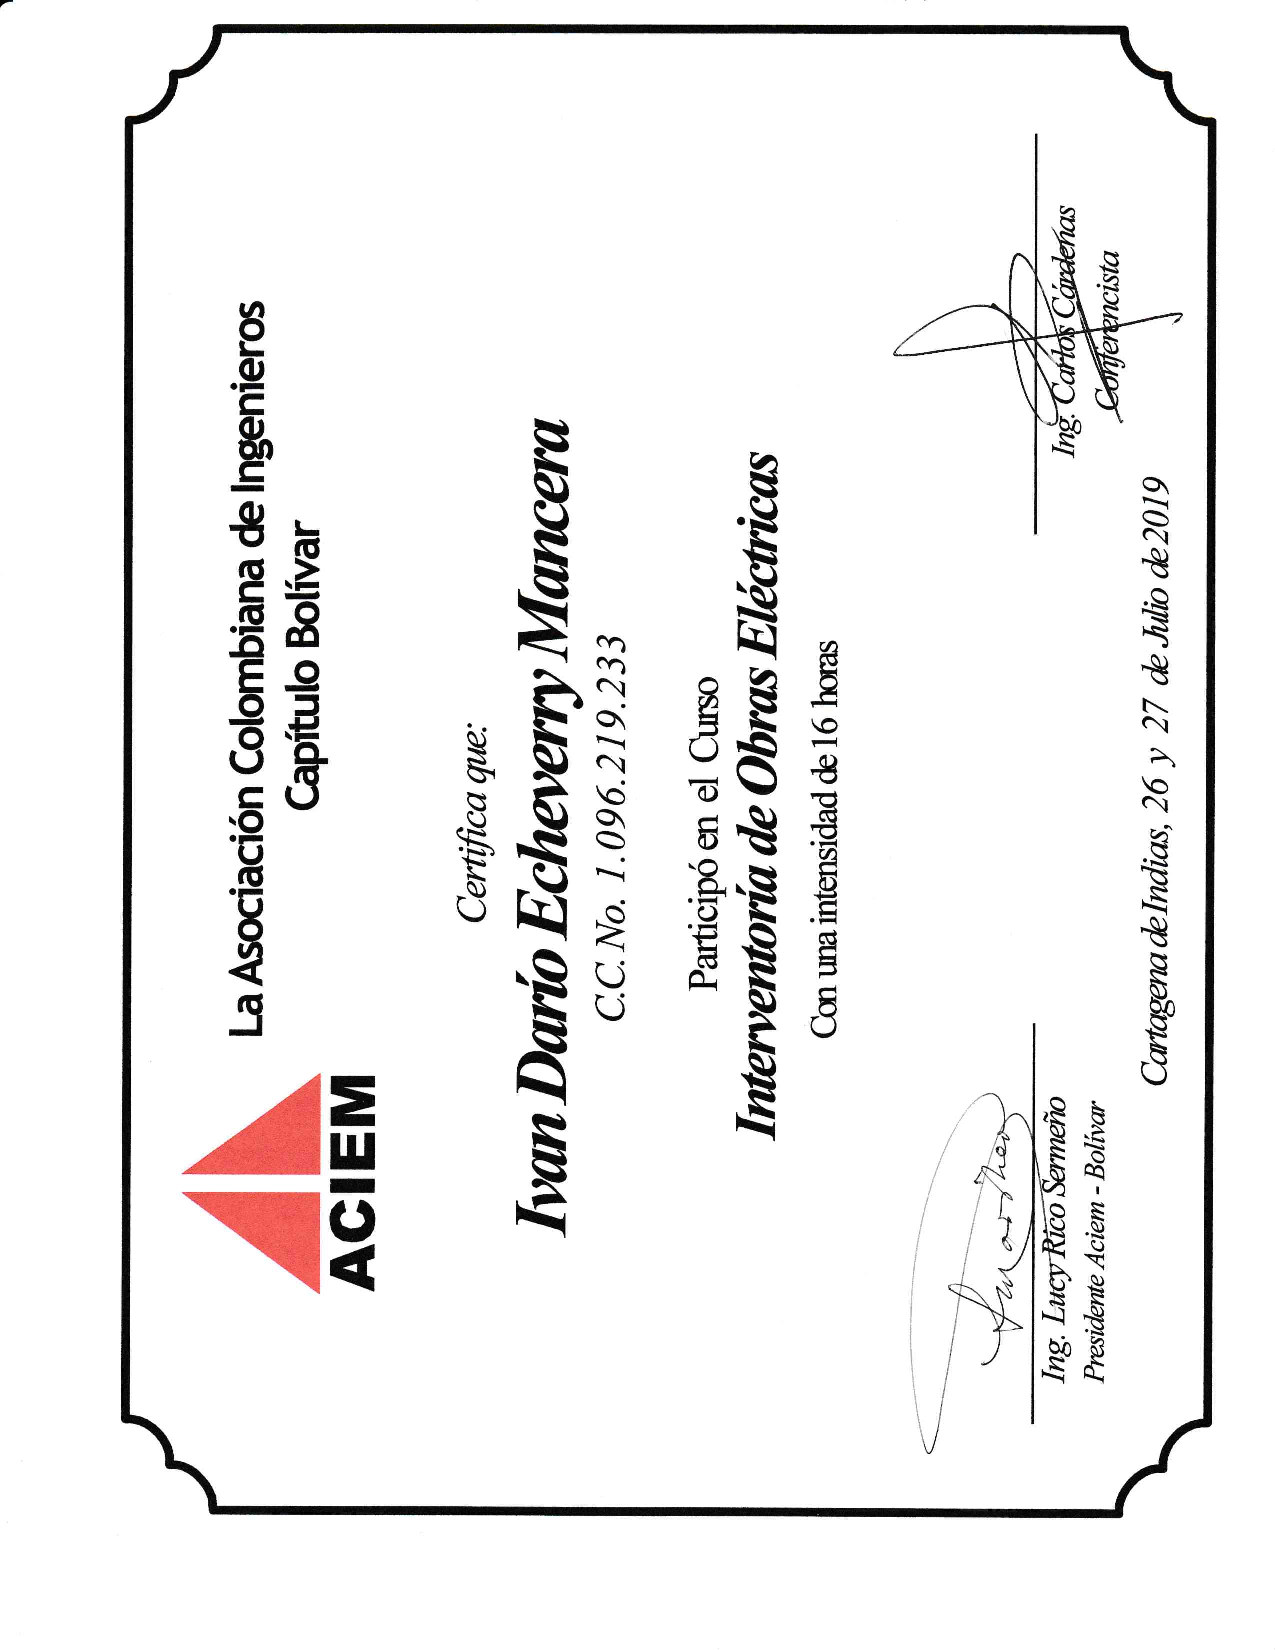
\includegraphics[width=1\textwidth]{ACIEM_Interventoria_en_Obras_Electricas.pdf}
%\caption{Certificado Curso Interventoria de Obras Eléctricas ACIEM.}
%\label{fig:Certificado1}
%\end{figure*}

%\newpage
%\begin{figure*}
%\centering
%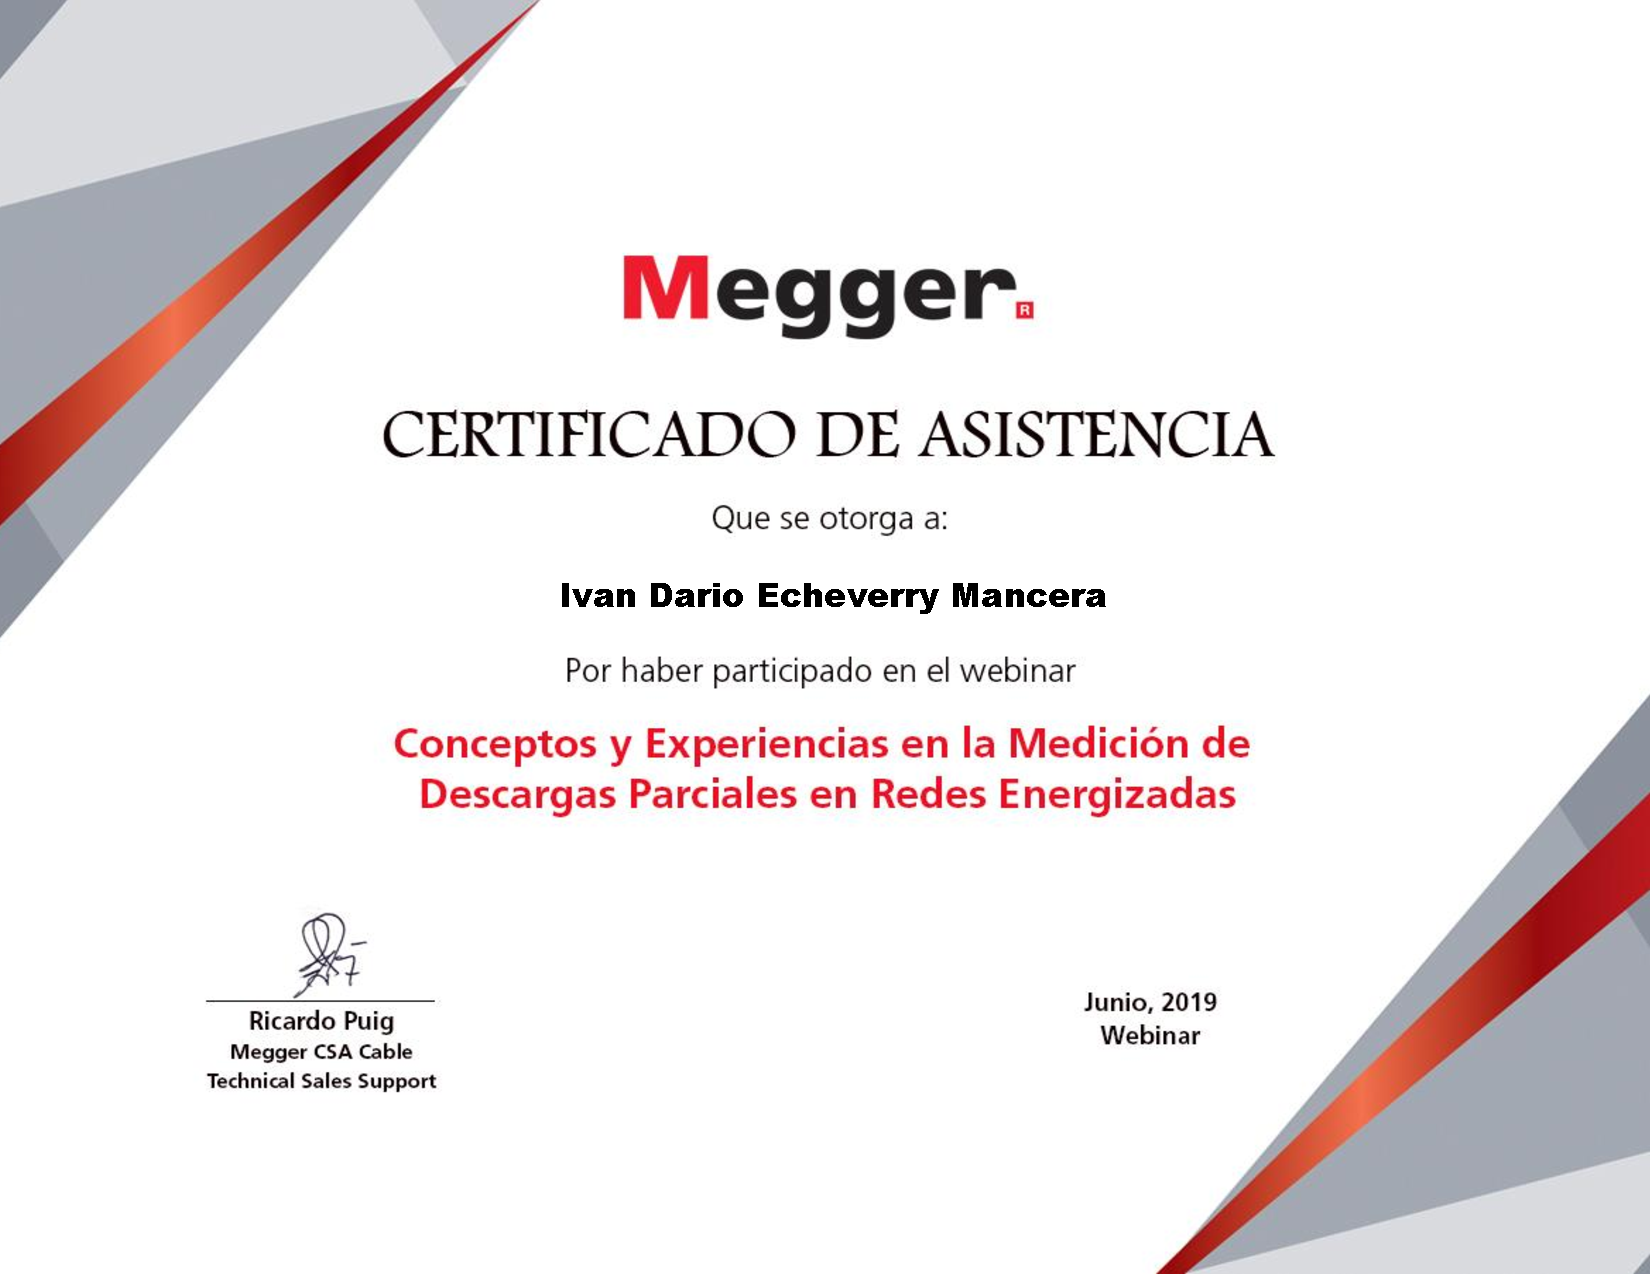
\includegraphics[width=1\textwidth]{certificadoMeggerDP.pdf}
%\caption{Certificado de asistencia webinar Megger.}
%\label{fig:Certificado1}
%\end{figure*}

%\newpage
%\begin{figure*}
%\centering
%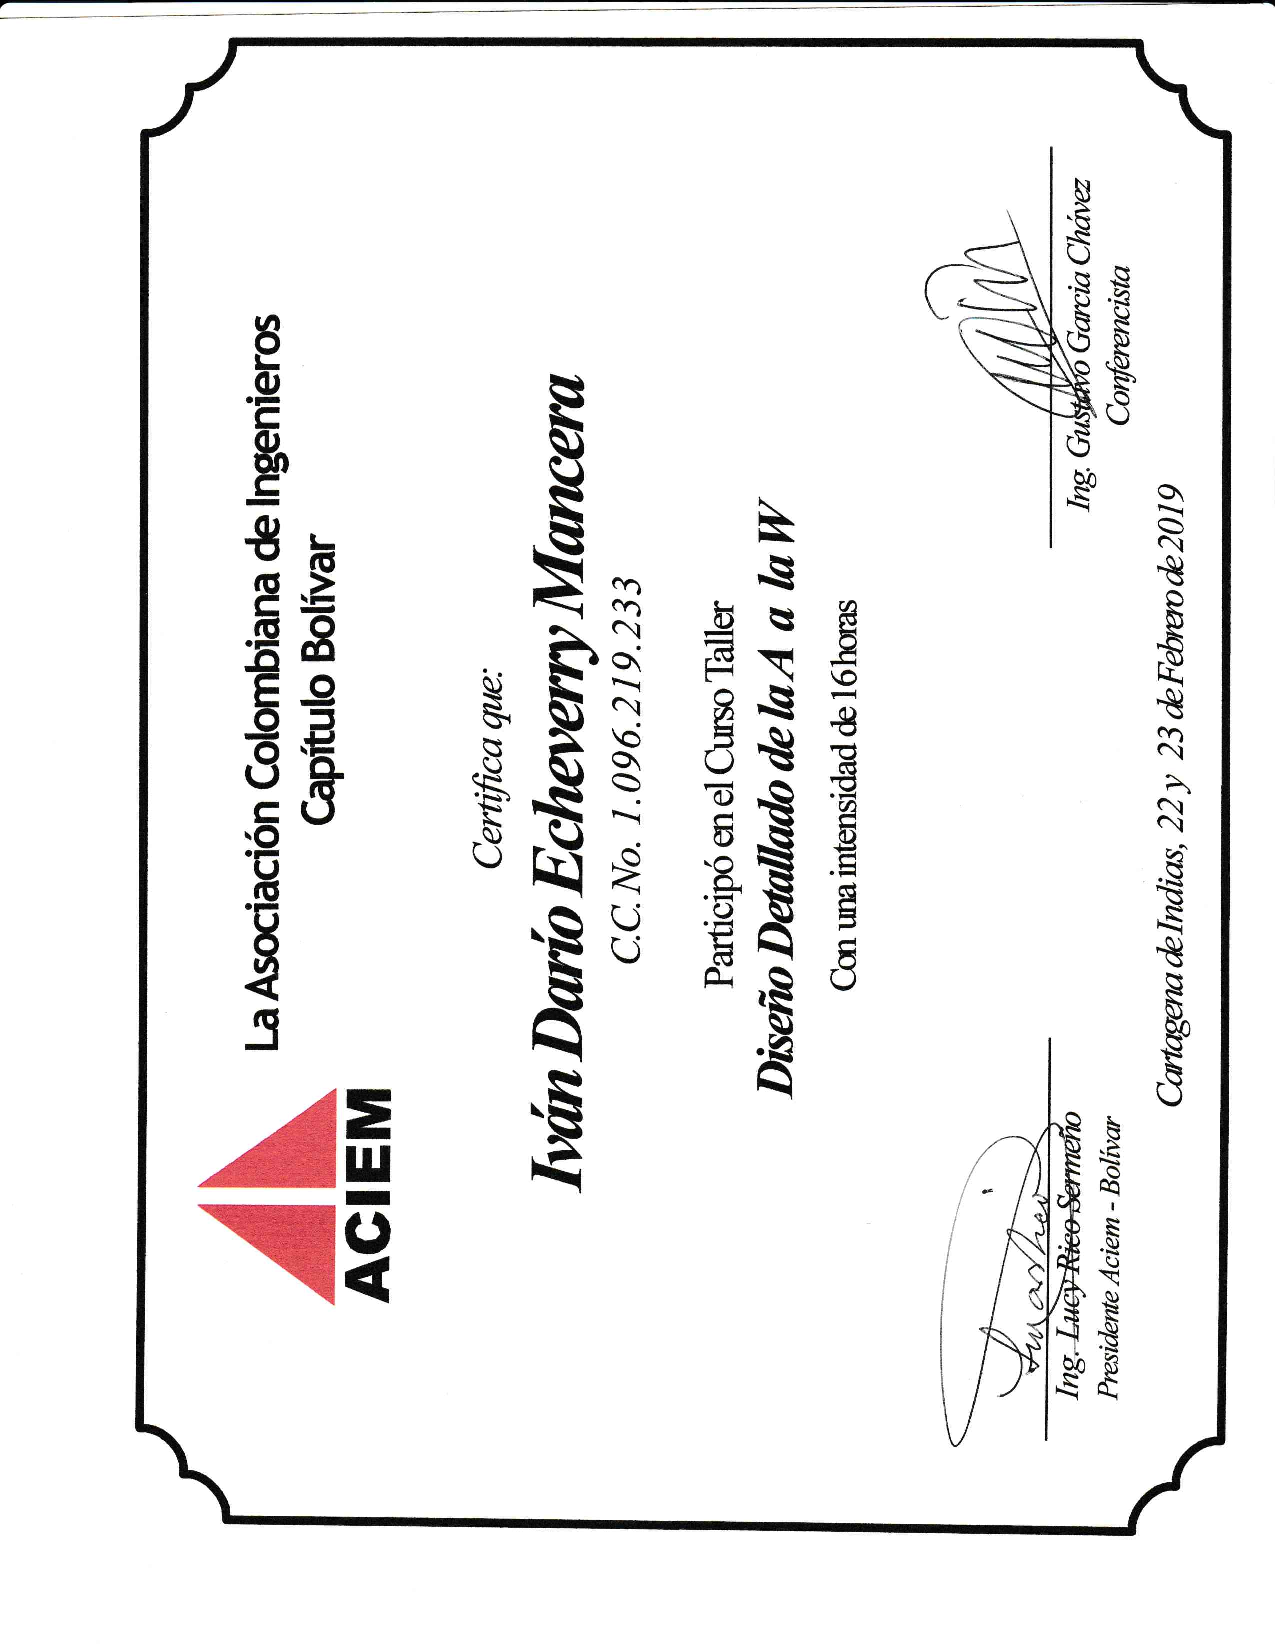
\includegraphics[width=1\textwidth]{ACIEM_Disenio_electrico_de_la_A_a_la_W.pdf}
%\caption{Certificado Curso Interventoria de Obras Eléctricas ACIEM.}
%\label{fig:Certificado1}
%\end{figure*}

\end{document}